% !TEX TS-program = pdflatex
% !TEX encoding = UTF-8 Unicode
% ORIGIN URL
% {{{ setup

\documentclass[11pt,twoside]{article}

\usepackage[utf8]{inputenc}

\usepackage[pdftex,
            pdftitle={Dispatching and Reconstructing SMT Proofs Through Reusable LambdaPi-modulo rewriting Encodings},
            pdfsubject={SMT, LambdaPi-modulo rewriting, Proof Reconstruction},
            pdfkeywords={SMT, Alethe, LambdaPi-modulo rewriting, proof assistants},
            pdfcreator={pdflatex},
            breaklinks]{hyperref}

% \usepackage{sectsty}
% \allsectionsfont{\sffamily\mdseries\upshape}

\usepackage[a4paper,margin=2.5cm,headheight=13.6pt]{geometry}
\usepackage{fancyhdr}
\pagestyle{fancy} % options: empty, plain, fancy
\renewcommand{\headrulewidth}{0pt}
\lhead{}\chead{}\rhead{}
\lfoot{}\cfoot{\thepage}\rfoot{}
\newcommand{\hide}[1]{}

\usepackage{url}

\usepackage{cite}

\usepackage{placeins}
\usepackage{subcaption}
\usepackage{multirow}
\usepackage{appendix}

\usepackage{xcolor}
\definecolor{dkgreen}{rgb}{0,0.6,0}
\definecolor{gray}{rgb}{0.5,0.5,0.5}
\definecolor{mauve}{rgb}{0.58,0,0.82}
\hypersetup{
    colorlinks,
    citecolor=black,
    filecolor=black,
    linkcolor=black,
    urlcolor=black
}

\usepackage{listings}
\lstdefinelanguage{none}{
  identifierstyle=
}
\newcommand{\lstNone}{
    \lstset{language=none,
            numbers=left,
            showstringspaces=false,
            numberstyle=\tiny\color{gray},
            numbersep=5pt,
            breaklines=false,
            basicstyle=\scriptsize\ttfamily}
}

\newcommand{\lstC}{
    \lstset{language=C,
            numbers=left,
            showstringspaces=false,
            numberstyle=\tiny\color{gray},
            keywordstyle=\color{blue},
            commentstyle=\color{dkgreen},
            stringstyle=\color{mauve},
            numbersep=5pt,
            breaklines=false,
            basicstyle=\small\ttfamily}
}

\lstdefinelanguage{LambdaPimodulorewriting}{
  keywords={symbol, constant, rule, TYPE, notation, infix, right, left},
  sensitive=true,
  morecomment=[l]{//},
  morestring=[b]",
  literate={→}{{$\to$}}1 {↪}{{$\hookrightarrow$}}1
}
\newcommand{\lstLambdaPimodulorewriting}{
    \lstset{language=LambdaPimodulorewriting,
            numbers=left,
            showstringspaces=false,
            numberstyle=\tiny\color{gray},
            keywordstyle=\color{blue},
            commentstyle=\color{dkgreen},
            stringstyle=\color{mauve},
            numbersep=5pt,
            breaklines=false,
            basicstyle=\small\ttfamily}
}

\usepackage{graphicx}
\usepackage{tikz}
\usetikzlibrary{shapes, shapes.arrows}

\usepackage{amsmath}
\usepackage{amssymb}
\usepackage{centernot}
\newcommand{\indep}{\perp\!\!\!\perp} % Define the independent symbol
\newcommand{\nindep}{\centernot{\indep}} % Define the not-independent symbol
\newcommand{\nimplies}{\centernot{\implies}} % Define the not-implies symbol
\newcommand{\niff}{\centernot{\iff}} % Define the not-iff symbol
\newcommand{\G}{\mathcal{G}}
\newcommand{\E}{\mathcal{E}}
\newcommand{\V}{\mathcal{V}}

\usepackage{siunitx}
\let\DeclareUSUnit\DeclareSIUnit
\let\US\SI
\DeclareUSUnit\ounce{oz}
\DeclareUSUnit\foot{ft}
\DeclareUSUnit\inch{in}
\DeclareUSUnit\mil{mil}
\DeclareSIUnit\dBi{dBi}

% Glossary support (uncomment and add entries when needed)
% \usepackage{glossaries}
% \makenoidxglossaries

\newcommand{\HRule}[1]{\rule{\linewidth}{#1}}

\newcommand{\TODO}[1]{[\textbf{TODO} \textsl{#1}]}

% \newcommand*{\ShowAbstract}{} % Uncomment to show the Abstract.
% \newcommand*{\ShowGlossary}{} % Comment to hide the Glossary.
% \newcommand*{\ShowAppendix}{} % Comment to hide the Appendix.

\author{Tiago Campos Ferreira\\\texttt{tiago-campos@ufmg.br}}

\title{$\lambda\Pi$-SMT: Dispatching and Reconstructing SMT Proofs Through Reusable $\lambda\Pi$-modulo encodings}

\date{}

% }}} setup

\begin{document}
% \sffamily % Commented out to use default Computer Modern serif font.

% {{{ prolog

\maketitle

% Abstract - uncomment ShowAbstract in preamble to display
\ifdefined\ShowAbstract \begin{abstract}
% TODO: Write abstract
\end{abstract} \fi

% }}} prolog

% ============================================================================
\section{Summary}
% ============================================================================

SMT solvers are widely used to decide the satisfiability of logical formulas modulo theories (e.g. arithmetic, bit vectors). When a solver produces a proof, its result can be independently validated through a proof certificate. One approach to validate such certificates is to reconstruct and check them inside a proof assistant.
Some existing approaches rely on the $\lambda\Pi$ logical framework as a unifying basis for proof checking \cite{coltellacci24smt}.
However, dispatching problems to SMT solvers and reconstructing proofs still requires proof-assistant specific encodings to the SMT-LIB format \cite{smtlib}.
A central challenge lies in encoding the proof calculi of certificates produced by SMT solvers, which leads to duplicated efforts across systems and significantly limits interoperability among SMT solvers, their proof formats, and target proof assistants.

This PhD proposal focuses on the problem of dispatching SMT problems and reconstructing proof obligations in multiple proof assistants using a shared intermediate framework.
We propose $\lambda\Pi$-SMT, a collection of meta-theorems and rewrite rules in $\lambda\Pi$ intended to factor out common proof-theoretic components of SMT reasoning.
The goal is to enable proof assistants with an existing $\lambda\Pi$ interface to reuse a common pipeline for SMT problem dispatching and proof reconstruction, reducing the need for repeated assistant-specific encodings.
In addition, we aim to extend existing work on translating Alethe proofs to $\lambda\Pi$ by supporting further SMT theories, such as bit vectors and strings. 

This extension focuses on incorporating additional, well-established SMT theories into the $\lambda\Pi$-SMT framework. 
While such theories are central to modern SMT solvers, they are still not uniformly supported across proof assistants with support for SMT proof discard, in the sense that their internal encodings are not well mapped to the SMT theories.
By providing a common $\lambda\Pi$-based interface for these theories, our tool enables their reuse in multiple proof assistants, avoiding direct interaction with low-level SMT proof formats and eliminating the need for assistant-specific theory encodings.

% ============================================================================
\section{Context}
% ============================================================================

SMT solvers are powerful tools for checking satisfiability of logical formulas modulo theories.
However, given the complexity of their algorithms and optimizations, their results can be questioned in the absence of proofs of correctness.
One way to increase confidence in their results is to mechanically verify their entire codebase, but this is often impractical: codebases are large, decision procedures and heuristics are complex to formalize, and maintaining the formalization as the solver evolves incurs significant costs.

A more practical approach is proof logging where a reasoner emits a proof artifact justifying its output, enabling independent verification \cite{barrett2015proofs}.
Successful examples of proof logging include the SMT solvers veriT \cite{verit2013} and cvc5 \cite{cvc5}.
Both support the Alethe proof format \cite{alethe2020}, which is designed to justify unsatisfiability results.
Alethe has an SMT-LIB-like \cite{smtlib} syntax (Figure~\ref{fig:alethe-example}) and natively supports the most common SMT theories.
Its fine-grained proof format makes it feasible to translate Alethe proofs into proof assistants such as Lean \cite{mohamed2025leansmtsmttacticdischarging} and Isabelle \cite{lachnitt_et_al:LIPIcs.ITP.2025.26}.

\begin{figure}[!ht]
\lstNone
\begin{lstlisting}
....
(step t10891.t1.t5.t12 (cl (not (and (< -1 0) (>= (s_count 3) 3))) (<= (* -1 (s_count 3)) (* -1 3)))
    :rule implies :premises (t10891.t1.t5.t11))
(step t10891.t1.t5.t13 (cl (and (< -1 0) (>= (s_count 3) 3)) (not (< -1 0)) (not (>= (s_count 3) 3))) 
   :rule and_neg)
(step t10891.t1.t5.t14 (cl (= (= (< -1 0) true) (< -1 0)))
    :rule equiv_simplify)
...
\end{lstlisting}
\caption{A real example extracted from an Alethe proof.}
\label{fig:alethe-example}
\end{figure}


The proof system inside the proof certificates can also be verified using a proof assistant, where the instances of rules are proved to be correct.
This differs from merely reconstructing a proof via proof logging.
Reconstructing a proof using proof logging is the task of translating the reasoning of the proof, for example, a SMT certificate, to other proof systems. That also means that they can fail to be reconstructed, when there is a mismatch between the proof format of the SMT solver and the proof assistant, or when the proof is incorrect.
Checking that they are correct requires a formalization of the proof system used by the SMT solver inside the proof assistant.
Examples of such approach include proving the step rules of Alethe in Dedukti \cite{alessio} and proving the correctness of the rules used in CVC5 in Isabelle \cite{LFA24}.
For example, one may want to prove that a certain rewriting step is correct: given a decidable equality and a Boolean expression $a$, can we derive $(= (= a\:true)\:a)$?
This is one of the rules used (equiv\_simplify \cite{alethe2020}) in Figure \ref{fig:alethe-example}, proved correct by Alessio et al. \cite{alessio} in $\lambda\Pi$-modulo rewriting.

Encoding semantics in a logical framework such as the $\lambda\Pi$-calculus modulo rewriting enables the representation of different proof systems via rewriting rules \cite{alessio}.
This is particularly useful because shallow embeddings of proof systems typically guarantee better integration. This means that we use the framework's logic to directly represent the semantics of the encoded logic, unlike deep embeddings that encode the proof system rules as algebraic data types and logical relations \cite{benzmueller2025faithful}.
With shallow embeddings in $\lambda\Pi$-modulo rewriting, we enjoy substitution, rewriting, and other meta-theoretical properties of the framework for free. For example, Alessio et al. \cite{alessio} translate Alethe proofs to Lambdapi \cite{hondet20fscd}, a logical framework that extends the $\lambda\Pi$-calculus with rewrite rules, and check their correctness with Lambdapi.
Moreover, Lambdapi proofs can be translated to other proof assistants such as Rocq and Lean \cite{thire18lfmtp,LPAR2024:Translating_HOL_Light_proofs}.

But still a gap remains in connecting SMT solvers to proof assistants.
While we are able to reconstruct Alethe certificates in $\lambda\Pi$-modulo, we need to establish a specific encoding for each proof assistant to dispatch a problem for an SMT solver and reconstruct the proof.
The typical pipeline converts the SMT problem to first-order logic using an encoding specific to each proof assistant, as done in Isabelle \cite{sleddehammer} and in Lean \cite{leansmt}.
This results in duplicated efforts to encode SMT theories for each proof assistant, the main challenge being here to reconstruct the proof in the original proof assistant.
Once we use a certain kind of encoding we still need to get the information back and preserve their meta-theoretical properties to the target proof system, so it is usually a more laborious task that may require a set of lemmas and strategies to match the same reasoning of the proof system used in the certificate \cite{leansmt}.

Consider an encoding of a higher-order formula $\phi$ in a proof assistant $A$, and let $F: \phi \rightarrow \phi'$ denote the mapping from a proof in higher-order logic to an SMT first-order logic proof object.
While $\phi'$ may be incomplete in the sense that some higher-order properties are lost in translation, $\phi'$ must imply any reconstructable truth in $\phi$, so any meta-encoding in $\phi'$ must correspond to a well-defined axiom or inference rule in $A$ related to $\phi$.
Now consider a mapping from $A$ to $\lambda\Pi$-modulo rewriting, denoted $L_A: \phi \rightarrow \phi_{LP}$. This mapping is faithful and complete, establishing a clear isomorphism, so it does translate any term, program or proof object. The current strategy sends $\phi'$ to the SMT solver, generates an Alethe $\pi'$ certificate translated to $\lambda\Pi$-modulo rewriting, and reconstructs the proof in $A$ directly from $\pi'$.
So we can still check the validity of $\phi'$ in $\lambda\Pi$-modulo rewriting, but we cannot universally reconstruct the proof in $A$ if we do not have a specific interface for $A$ to the SMT proof format.
We propose a different approach: translate $\phi_{LP}$ to SMT first-order logic problem, convert back to $\lambda\Pi$-modulo rewriting and then using the inverse mapping to obtain the proof object again by $L_A^{-1}$.

\hide{
Indeed, consider a formula $\phi_A$ in a proof assistant $A$ and let
$\phi'_{SMT}$ be a translation of $\phi_A$ in the SMT logic. Because
proof assistant logics are usually more expressive than the SMT logics
(higher-order logic or dependent type theory vs first-order logic),
this translation is generally not complete in the sense that not all
formulas provable in $A$ are provable by a SMT solver. On the other
hand, translations are designed so that one can obtain a proof of
$\phi_A$ from a proof of $\phi'_{SMT}$.
%
Let $L_A$ be a faithful and complete mapping of $A$ to Lambdapi.  The
current strategy sends $\phi'_{SMT}$ to a SMT solver, gets back an
Alethe proof $\pi'_{Alethe}$, translates it to a Lambdapi proof
$\pi'_{LP}$ of $\phi'_{SMT}$, and then to a proof of $\phi'_{SMT}$ in
$A$ by applying $L_A^{-1}$. We can check the validity of $\pi'_{LP}$
in Lambdapi but we cannot universally reconstruct a proof in $A$ if we
do not have a specific interface in $A$ to the SMT proof format.
%
We propose a different approach: translate $\phi_A$ to $\phi_{LP}$ in
Lambdapi, transform the formula $\phi_{LP}$ that is the Lambdapi
theory for $A$ to a formula $\phi'_{LP}$ that is in the Lambdapi
theory of SMT, and prove in Lambdapi that $\phi_{LP}$ is provable
whenever $\phi'_{LP}$ so is. Then, send $\phi'_{LP}$ to a SMT solver,
get back an Alethe proof $\pi'_{Alethe}$, translate it to a Lambdapi
proof $\pi'_{LP}$, get in Lambdapi a proof $\pi_{LP}$ of $\phi_{LP}$,
and translate it back to a proof of $\phi_A$ in $A$ using $L_A^{-1}$.
}

We plan to map terms to SMT formulas that faithfully encode only the fragment of the proof system encoded in $\lambda\Pi$.
To this end, we must establish a collection of facts that reconstruct the reasoning performed by SMT theories.
These facts must still be processed by the proof assistant $A$'s pipeline. For this purpose, we plan to design a gentle encoding that we already translate to and reconstruct in
from the SMT solver, allowing the proof assistant  $A$ to consume it directly by its interface with $\lambda\Pi$.
For example in Figure \ref{fig:LambdaPirewritingexample}, we give hints to the LambdaPi interface of how each rewrite rule maps to a certain SMT step.

Note that the hints must provide information for both the dispatch and reconstruction pipelines of SMT. 
When a proof obligation involves these rules, we can automatically dispatch the problem using a theory-appropriate encoding for the SMT solver.
Conversely, when a proof certificate contains these rules, we can reconstruct the proof in the proof assistant using the information supplied by the reconstruction hints.

We still emphasize that the interface of $\lambda\Pi$-modulo with the proof assistant must be designed using these rules, but once the interface is done, the user does not need to interact with the SMT proof format directly.

\begin{figure}[!ht]
\lstLambdaPimodulorewriting
\begin{lstlisting}
symbol Cod: TYPE;
symbol IntCod : Cod;
symbol BitVectorCod : Cod;
symbol UF_Cod : Cod;

// Very Simple Universe for SMT types
symbol SimpleUnivSMT : Cod → TYPE;

// Natural numbers
constant symbol Nat : TYPE;
constant symbol zero : Nat;
constant symbol suc : Nat → Nat;

constant symbol pos    : Nat → SimpleUnivSMT IntCod;
constant symbol negsuc : Nat → SimpleUnivSMT IntCod;

// Addition on integers
symbol + : SimpleUnivSMT IntCod → SimpleUnivSMT IntCod → SimpleUnivSMT IntCod;
notation + infix right 6 with desugar SMT("+");
// Where caseSMT_Int_Add is a friendly inductive encoding
rule x + y ↪ caseSMT_Int_Add($x, $y) with reconstruction SMT("int-add");
// x + 0 = x
rule $x + pos zero ↪ $x with reconstruction SMT("int-add-zero-right");

\end{lstlisting}
\caption{A high-level abstraction of communicating SMT-LIB in $\lambda\Pi$-modulo rewriting.}
\label{fig:LambdaPirewritingexample}
\end{figure}

% ============================================================================
\section{PhD Objectives}
% ============================================================================

A good implementation of $F$ converts the encoding from $A$ to the closest SMT-supported theory. This requires a set of lemmas in $A$ corresponding to those used by the SMT solver's theory engine.
For instance, when reconstructing a proof, a database of meta-theorems matching the theory engine guides the reconstruction \cite{Bhme2012ProvingTO}.

We propose \textit{$\lambda\Pi$-modulo rewriting-SMT}, a database of meta-theorems in $\lambda\Pi$-modulo rewriting sufficient for dispatching SMT problems across different proof assistants.
Since $\lambda\Pi$-modulo rewriting has a small core, we aim to preserve this property when designing the meta-theorems. For example, in hol2dk \cite{Blanqui2024HOLLightToCoq},
inductive types for first-order terms in HOL-Light (such as product types and natural numbers) are translated between HOL and Rocq by proving that their shallow embeddings are equivalent.

To support different proof assistants, the differences in their type systems must be considered.
The rewrite rules and encoding should be designed for translation across different settings of universe levels, inductive principles, and similar features.
Since SMT theories are typically first-order, this considerably simplifies the task of the user who wants to map their definitions into $\lambda\Pi$-modulo rewriting-SMT.
In fact, the user only needs to use the meta-theorems corresponding to the SMT theories or map their definitions to existing ones in $\lambda\Pi$-modulo rewriting-SMT.
This can be done using different translation tools already available, such as hol2dk \cite{Blanqui2024HOLLightToCoq}, the K framework to Dedukti \cite{ledein:hal-03895834}, and others as described in the translation pipeline in Figure \ref{fig:translation-pipeline}.

\begin{figure}[!ht]
    \centering
    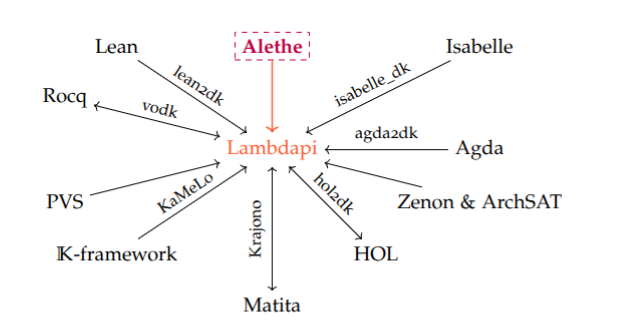
\includegraphics[width=0.8\linewidth]{img/image.png}
    \caption{Translation pipeline from proof assistants to $\lambda\Pi$-modulo rewriting (Source: Alessio's PhD \cite{alessio}).}
    \label{fig:translation-pipeline}
\end{figure}

We also plan to reuse Alessio's work \cite{alessio} in this context, allowing users to map Alethe definitions into their proof assistants without interacting directly with Alethe certificates.

% ============================================================================
\section{Methods and Workplan}
% ============================================================================

This proposal builds on existing work on Alethe proof reconstruction in $\lambda\Pi$-modulo rewriting:

\begin{itemize}
    \item \textbf{Extend theory support:} Extend Alessio's work to handle bit-vector and array theories by translating the cvc5 calculus for bit-vectors and strings into $\lambda\Pi$-modulo rewriting.
    \item \textbf{Design the meta-theorem framework:} Design a framework mapping $\lambda\Pi$-modulo rewriting meta-theorems to SMT theories, supporting problem dispatching and proof reconstruction in different proof assistants from Alethe certificates.
    \item \textbf{Proof of concept:} Develop a proof of concept using Lean as the target proof assistant.
\end{itemize}

% }}} sec:SECTION

% {{{ epilog

\clearpage
\addcontentsline{toc}{section}{References}
\bibliography{main}{} % main.bib
\bibliographystyle{plain}

% Glossary disabled - uncomment when glossary package is enabled
% \ifdefined\ShowGlossary
%     \addcontentsline{toc}{section}{Glossary}
%     \printnoidxglossary[sort=letter]
% \fi

% Appendix disabled - uncomment and add content when needed
% \ifdefined\ShowAppendix \begin{appendices}
%     \addappheadtotoc
%     \appendixpage
%     % Add appendix sections here
% \end{appendices} \fi

% }}} epilog

\end{document}
